\hypertarget{utils_8inc}{
\section{include/utils.inc File Reference}
\label{utils_8inc}\index{include/utils.inc@{include/utils.inc}}
}
Helpful Utilities. 

\subsection*{Functions}
\begin{CompactItemize}
\item 
\hyperlink{utils_8inc_846199262ea0cd07e0531f38d26dd9b3}{fget} (\$url)
\end{CompactItemize}


\subsection{Detailed Description}
Helpful Utilities. 

These utilities are suitable to be included in any file by calling the file as follows: 

\begin{Code}\begin{verbatim} require_once 'utils.inc'
\end{verbatim}
\end{Code}

 

Definition in file \hyperlink{utils_8inc-source}{utils.inc}.

\subsection{Function Documentation}
\hypertarget{utils_8inc_846199262ea0cd07e0531f38d26dd9b3}{
\index{utils.inc@{utils.inc}!fget@{fget}}
\index{fget@{fget}!utils.inc@{utils.inc}}
\subsubsection{\setlength{\rightskip}{0pt plus 5cm}fget (\$ {\em url})}}
\label{utils_8inc_846199262ea0cd07e0531f38d26dd9b3}


Download a {\bf text} file using cURL \begin{Desc}
\item[Parameters:]
\begin{description}
\item[{\em \$url}]The URL to download \end{description}
\end{Desc}
\begin{Desc}
\item[Returns:]A string containging the text file \end{Desc}


Definition at line 16 of file utils.inc.

Referenced by getImages().

\begin{Code}\begin{verbatim}16                     {
20   $curl = curl_init($url);
21 
22   curl_setopt_array($curl, array(
23     CURLOPT_REFERER => $_ENV['SCRIPT_URI'],
24     CURLOPT_FAILONERROR => TRUE,
25     CURLOPT_RETURNTRANSFER => 1,
26     CURLOPT_CLOSEPOLICY => CURLCLOSEPOLICY_LEAST_RECENTLY_USED,
27   ));
28 
32   $file = curl_exec($curl);
33   curl_close($curl);
34 
35   return $file;
36 }\end{verbatim}
\end{Code}




Here is the caller graph for this function:\nopagebreak
\begin{figure}[H]
\begin{center}
\leavevmode
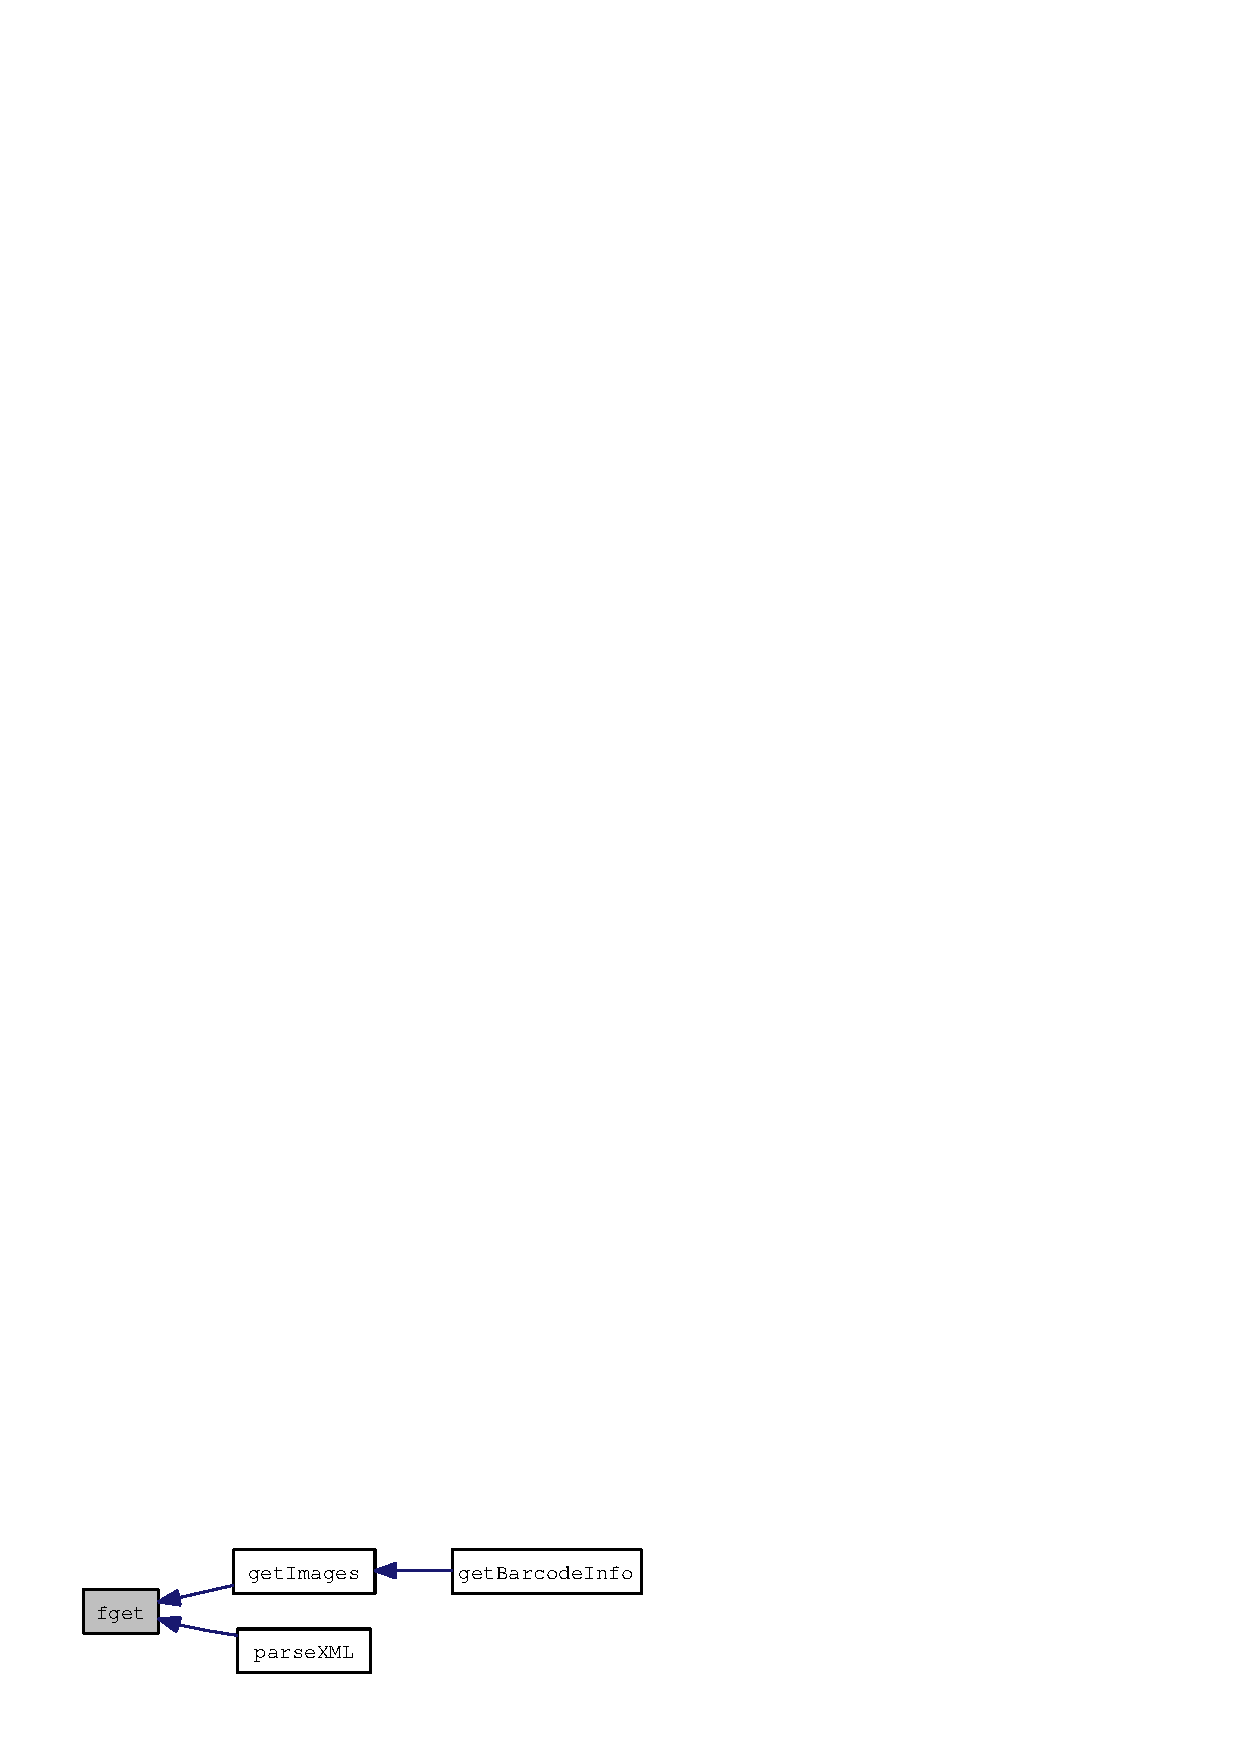
\includegraphics[width=156pt]{utils_8inc_846199262ea0cd07e0531f38d26dd9b3_icgraph}
\end{center}
\end{figure}
